\chapter{実験}
\label{chap:experiment}


\section{実験の目的}
\label{sec:purpose}

本実験を行うことで、蓄電池を用いた電力融通手法による電力制約下での性能向上効果を見積もる。蓄電池の特性としては\ref{sec:formularization}節で述べたような理想的な特性を仮定する。また\ref{sec:curb}節で述べたように、蓄電池を用いた電力融通による電力制約下での性能向上が起こる場合には3つのケースがある。そこで、それぞれのケースがどの程度の効果をもたらしているかを評価・考察する。



\section{実験方法}
\label{sec:method}

本手法を用いた性能向上を実現するためには以下の3つの段階を踏む必要がある。

\begin{enumerate}
\item ユーザがアプリケーションのソースコードに埋め込んだフェーズ区切り文を読み取り、アプリケーションを分割する。
\item 分割されたフェーズそれぞれについて電力−実行時間曲線を求める
\item 分割されたフェーズに対する電力融通問題を解く
\end{enumerate}

まず、1段階目について述べる。実際に\ref{sec:phase2}節のように書かれたソースコードからフェーズ区切り文を読み取るのはコンパイラレベルでの実装が必要となり困難である。そのため、本実験ではそのフェーズに入ったもしくは出た時刻をログとして出力する自作関数をソースコードに埋め込むことによって、その代わりとした。また、今回実験に利用したアプリケーションは自作のものではないので、ソースコードを読んでどの部分がフェーズの区切りであるかを完全に知ることは困難であった。そこで簡単のため、並列処理部分と逐次処理部分のみをソースコードから判別してフェーズ分割を行った。そして、プロセッサの取りうる全てのDVFSパターンについてアプリケーションを実行し、ログファイルを得た。ただし表\ref{tbl:parsec}に示したアプリケーションのうち、QT Clusteringのみは並列実行の中に2つのフェーズがあったため、全体で並列処理1・並列処理2・逐次処理の3フェーズに分割した。

次に2段階目である。ここでは1段階目で得たログファイルから、それぞれのフェーズについて全てのDVFSパターンにおける平均電力と実行時間を得ることができる。それを用いてそれぞれのフェーズの電力−実行時間曲線を計算した。ただし実際にはDVFSパターンは有限であるので、電力−実行時間曲線は図\ref{fig:discrete_power_time}のようになった。

\begin{figure}[t]
 \begin{center}
  \includegraphics[width=118mm]{discrete_power_time.eps}
 \end{center}
 \caption{離散的な周波数しか取れない場合の電力−実行時間曲線}
 \label{fig:discrete_power_time}
\end{figure}

最後に3段階目は、\ref{sec:algorithm}節で述べたように得られた電力−実行時間曲線から総当たりで最適なDVFS設定値を見つけた。

また\ref{sec:purpose}節で述べたように、本実験の目的には電力制約下での性能向上をもたらす3つのケースのそれぞれの効果を評価することも含まれる。しかし、ここまでの実験方法ではそれぞれケースの影響が入り交じった結果のみしか得られないため、それぞれのケースの効果を見積もることは困難である。そこで、ケース3の効果はプロセッサが離散的な周波数のみしか取ることができないことが原因であることに着目した。本実験の2段階目で得られた電力−実行時間曲線を式\ref{asm:model}に合うように補間することによって、連続な電力−実行時間曲線を求め(図\ref{fig:continuous_power_time})、ケース3の影響のみを切り分けて評価できるようにした。ただし完全に連続であると電力融通問題を総当たりで解くことができなくなるため、実際にはある程度の細かい間隔で補間することで連続的な曲線への近似とした。そして、3段階目では同様に総当たりで最適なDVFSの設定値を見つけた。この結果を周波数が離散的な場合の結果と比較するにより、ケース3の効果をケース1、2の効果とは切り分けて見積もることができる。

\begin{figure}[t]
 \begin{center}
  \includegraphics[width=118mm]{continuous_power_time.eps}
 \end{center}
 \caption{連続補間した場合の電力−実行時間曲線}
 \label{fig:continuous_power_time}
\end{figure}

用いたベンチマークアプリケーションは表\ref{tbl:parsec}の通りである。CPU並列のアプリケーションではCPUの電力のみ、GPU並列のアプリケーションであればGPUの電力のみを測定した。

\begin{table}[t]
\begin{center}\begin{tabular}{|c|c|c|}
\hline ワークロード名 & & 説明 \\
\hline PARSEC Canneal & CPU並列 & \shortstack{SAアルゴリズムを用いてルーティングコストが\\最小となるchipを設計する. }\\
\hline PARSEC Stream Cluster & CPU並列 & \shortstack{ストリーミングされる点列の\\オンラインクラスタリングを行う. }\\
\hline Rodinia mummergpu & GPU並列 & 深さ優先探索によりDNA塩基配列を求める\\
\hline SHOC QT Clustering & GPU並列 & \shortstack{クラスタメンバ間の相関が指定されたカットオフ値より\\高いことを保証するクラスタリング}\\
\hline \end{tabular} \caption{使用したベンチマークアプリケーションの詳細}\label{tbl:parsec}
\end{center}
\end{table}

\begin{table}[h]
    \centering
    \begin{tabular}{|c|c|c|}
        \hline
                     & 名称  &  周波数 (MHz) \\ \hline
        CPU          & Intel Core i7 4770 4コア & 800 - 3200   \\ \hline
        GPUs         & NVIDIA K20c 2496コア         & 324 - 758  \\ \hline
        MotherBoards & ASRock H87M & -- \\ \hline
        OS           & Ubuntu 13.04 &  -- \\ \hline
    \end{tabular}
    \caption{実験機の構成}
    \label{tab:machine-setup}
\end{table}



\section{結果}
\label{sec:result}

それぞれのアプリケーションの電力−実行時間曲線を図\ref{fig:canneal_power_time}、\ref{fig:streamcluster_power_time}、\ref{fig:mummergpu_power_time}、\ref{fig:qtclustering_power_time}に、スピードアップ曲線を図\ref{fig:canneal_speedup}、\ref{fig:streamcluster_speedup}、\ref{fig:mummergpu_speedup}、\ref{fig:qtclustering_speedup}に示す。ただし、スピードアップは以下のように定義される。

\begin{eqnarray}
スピードアップ =  1 - \frac{{\rm UPS}ありの場合のアプリケーション全体の実行時間}{{\rm UPS}なしの場合のアプリケーション全体の実行時間}
\end{eqnarray}


Cannealの電力−実行時間曲線は並列処理と逐次処理の電力消費の違いをよく表しており、並列処理の方が逐次処理より大きい電力を消費していることが分かる。Stream Clusterも同様の傾向は見て取れるが、Cannealとは違って逐次処理部分の実行時間が非常に短いことが特徴である。mummergpuのグラフを見ると、どのDVFS設定においても逐次処理部分の実行時間が変わらないことが分かる。これは\ref{sec:method}節で述べたようにGPU並列アプリケーションはGPUの電圧のみを測定しているため、CPUで演算をしている逐次処理部分はの実行時間はGPUの周波数に影響を受けないためである。QT Clusteringでは3つのフェーズがあり、mummergpu同様に逐次処理部分はDVFSの設定によらずほぼ同じ実行時間になっている。

次にスピードアップのグラフについてであるが、全体的に離散的な周波数しか取れない場合の方が、連続的に周波数を変化できる場合に比べて効果は大きかった。また離散的な場合は電力制約ごとにスピードアップの変動が大きく、大きくスピードアップする場合もあれば全くスピードアップしない場合もある。連続の場合では、離散的な場合のようにスピードアップの値が大きく変動することはなかったが、やはり電力制約に応じてある程度の変動は見て取れる。

\begin{table}[t]
\begin{center}\begin{tabular}{|c|c|}
\hline ワークロード名 & スピードアップ平均 \\
\hline PARSEC Canneal & 4.54\%\\
\hline PARSEC Stream Cluster & 0.56\%\\
\hline Rodinia mummergpu & 18.23\%\\
\hline SHOC QT Clustering & 15.89\%\\
\hline \end{tabular} \caption{スピードアップの算術平均(周波数が離散の場合)}\label{tbl:parsec}
\end{center}
\end{table}

\begin{table}[t]
\begin{center}\begin{tabular}{|c|c|}
\hline ワークロード名 & スピードアップ平均 \\
\hline PARSEC Canneal & 2.22\%\\
\hline PARSEC Stream Cluster & 0.02\%\\
\hline Rodinia mummergpu & 10.44\%\\
\hline SHOC QT Clustering & 2.50\%\\
\hline \end{tabular} \caption{スピードアップの算術平均(周波数が連続の場合)}\label{tbl:parsec}
\end{center}
\end{table}

\begin{figure}[t]
 \begin{center}
  \includegraphics[width=125mm]{canneal_power_time.eps}
 \end{center}
 \caption{Canneal 電力−実行時間曲線}
 \label{fig:canneal_power_time}
\end{figure}

\begin{figure}[t]
 \begin{center}
  \includegraphics[width=125mm]{canneal_speedup.eps}
 \end{center}
 \caption{Canneal スピードアップグラフ}
 \label{fig:canneal_speedup}
\end{figure}

\begin{figure}[t]
 \begin{center}
  \includegraphics[width=125mm]{streamcluster_power_time.eps}
 \end{center}
 \caption{Stream Cluster 電力−実行時間曲線}
 \label{fig:streamcluster_power_time}
\end{figure}

\begin{figure}[t]
 \begin{center}
  \includegraphics[width=125mm]{streamcluster_speedup.eps}
 \end{center}
 \caption{Stream Cluster スピードアップグラフ}
 \label{fig:streamcluster_speedup}
\end{figure}

\begin{figure}[t]
 \begin{center}
  \includegraphics[width=122mm]{mummergpu_power_time.eps}
 \end{center}
 \caption{mummergpu 電力−実行時間曲線}
 \label{fig:mummergpu_power_time}
\end{figure}

\begin{figure}[t]
 \begin{center}
  \includegraphics[width=122mm]{mummergpu_speedup.eps}
 \end{center}
 \caption{mummergpu スピードアップグラフ}
 \label{fig:mummergpu_speedup}
\end{figure}

\begin{figure}[t]
 \begin{center}
  \includegraphics[width=122mm]{qtc_power_time.eps}
 \end{center}
 \caption{QT Clustering 電力−実行時間曲線}
 \label{fig:qtclustering_power_time}
\end{figure}

\begin{figure}[t]
 \begin{center}
  \includegraphics[width=122mm]{qtc_speedup.eps}
 \end{center}
 \caption{QT Clustering スピードアップグラフ}
 \label{fig:qtclustering_speedup}
\end{figure}


\begin{figure}[t]
 \begin{center}
  \includegraphics[width=122mm]{canneal_speedup_continuous_modified.eps}
 \end{center}
 \caption{Canneal スピードアップグラフ(連続の場合のみ)}
 \label{fig:canneal_speedup_continuous}
\end{figure}

\begin{figure}[t]
 \begin{center}
  \includegraphics[width=122mm]{frequency_transition_canneal.eps}
 \end{center}
 \caption{Canneal 周波数の推移の様子(連続の場合)}
 \label{fig:frequency_transition_canneal}
\end{figure}

\begin{figure}[t]
 \begin{center}
  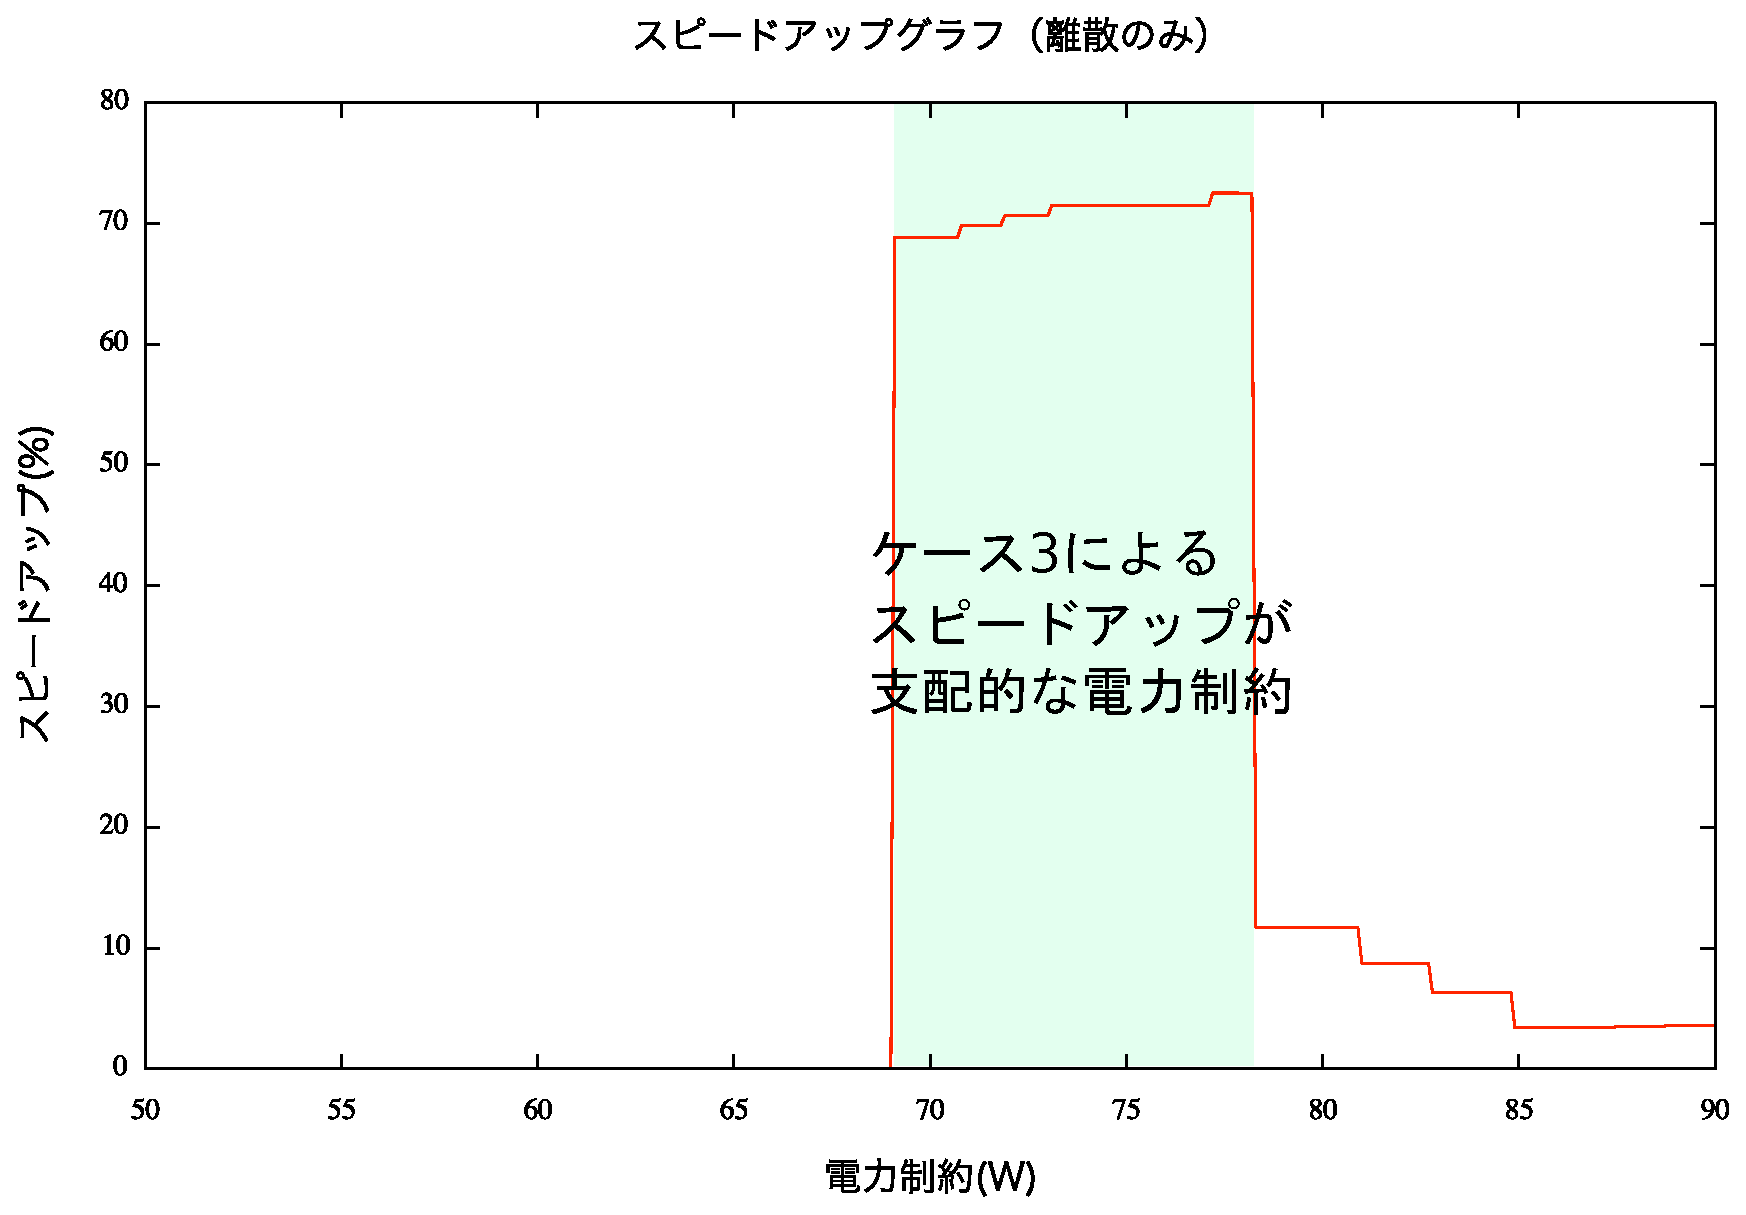
\includegraphics[width=123mm]{mummergpu_speedup_discreet_modified.eps}
 \end{center}
 \caption{mummergpu スピードアップグラフ(離散の場合のみ)}
 \label{fig:mummergpu_speedup_discreet}
\end{figure}

\begin{figure}[t]
 \begin{center}
  \includegraphics[width=123mm]{frequency_transition_mummergpu.eps}
 \end{center}
 \caption{mummergpu 周波数の推移の様子(離散の場合)}
 \label{fig:frequency_transition_mummergpu}
\end{figure}


\section{考察}
\label{sec:discussion}

4つのアプリケーションの中で、Stream Clusterのみは蓄電池を用いた電力融通にスピードアップがとても小さかった。これは、逐次処理部分の実行時間が並列処理部分の実行時間と比べて非常に短かったため、蓄電池が充放電する時間がほとんどなく、電力融通を上手く行うことができなかったためであると考えられる。

\subsection{周波数が連続的な値を取れる場合の考察}
\label{subsec:continuous}


連続的に周波数が変更できる場合にどのような周波数が最適解となっているかについて考察する。ここでは比較的説明のしやすい、Cannealの連続補間した場合の結果について説明する。

図\ref{fig:canneal_speedup_continuous}、\ref{fig:frequency_transition_canneal}はそれぞれ、周波数が連続的に変えられる場合のCannealの電力−実行時間曲線とスピードアップグラフである。図\ref{fig:canneal_speedup_continuous}を見ると、電力制約が17Wの部分からスピードアップが増加し始め、28W付近でピークに達しその後は減少していくのが分かる。

まず、電力制約が17Wより小さいときの最適周波数について考える。図\ref{fig:frequency_transition_canneal}を見ると分かるように、この範囲においては、逐次処理の周波数を下げて並列処理の周波数を上げている。つまり、逐次処理部分は電力を上げても実行時間があまり短縮されないフェーズであり、逆に並列処理部分は電力を上げることで実行時間が大きく短縮されるフェーズであったということである。ただしここで注意すべきは、蓄電池によって融通しているものは電力ではなくエネルギであるという点である。フェーズAで10Wで充電できたからといって、フェーズBで10Wで放電できるとは限らない。これはそれぞれのフェーズの実行時間が異なるため、充電できるエネルギに差が生じるためである。しかし、\ref{sec:formularization}節で述べたような理想的な蓄電池の場合にはフェーズAで10J充電できた場合はフェーズBで必ず10J放電することができる。つまり、それぞれのフェーズにかけるエネルギを微小変化させたときの、実行時間の短縮の大きさを見てやればよいことになる。これは、実行時間を実行エネルギで微分したものを正負逆転させたものに他ならない。これをエネルギ実行時間短縮率と呼ぶこととする。エネルギ実行時間短縮率は式\ref{asm:model}を用いて以下のように求められる。

\begin{eqnarray}
E &=& p \cdot T(p)\\
-\frac{dT}{dE} &=& -\frac{dT}{dp} \bigg/ \frac{dE}{dp}\\
&=& -\frac{1}{a_2 - \cfrac{a_0}{a_1}( p-a_2)^2} \label{asm:differential}
\end{eqnarray}

実際に17W以下の部分については、式\ref{asm:differential}の値がほぼ一致していた。つまりこの部分については、それぞれのフェーズのエネルギ実行時間短縮率の一致する部分が最適解となっている。また、この部分におけるスピードアップは0.5\%未満とかなり小さい。

次に17-28Wの部分について考える。図\ref{fig:frequency_transition_canneal}を見ると分かるように、17Wのときに、電力融通をしない場合の逐次処理部分での動作周波数が頭打ちになり、実行時間が短くならなくなる。一方で電力融通を行う場合には頭打ちになるのがもう少し遅く、頭打ちになってもその部分で余った電力を並列部分へ融通して周波数を上げることができるので、実行時間は短くなり続ける。そのため実行時間の差は開き続け、スピードアップが大きくなり続ける。

この電力制約における最適周波数での式\ref{asm:differential}の値を見ると、逐次処理の値の方が小さい。これは逐次処理の方がエネルギ実行時間短縮率が大きいことを意味しているため、もし逐次処理の周波数をさらに上げることができれば、並列処理部分での動作周波数を下げ、代わりに逐次処理部分では動作周波数を上げていたと予想される。

最後に28W以上の部分について考える。この部分についての説明は容易である。図\ref{fig:frequency_transition_canneal}から、28Wのときに電力融通を行っている場合には逐次処理・並列処理のどちらのフェーズも動作周波数が頭打ちになる。従って、電力融通をしている場合にはこれ以上実行時間を短縮する余地がない。一方で電力融通していない場合には、並列処理部分の動作周波数をまだ上げることができるため、実行時間が短縮されていく。結果としてスピードアップは減少していく。

以上それぞれのフェーズにおける考察より、プロセッサが連続的な周波数で動作できる場合にはエネルギ実行時間短縮率が高いフェーズから低いフェーズへできる限り電力を融通できるような充放電計画が最適となることが分かる。また、17W以下の部分のスピードアップを見れば分かるように、電力−実行時間曲線の特性の違いによって生じるエネルギ実行時間短縮率の違いを利用した電力融通だけでは効果は小さい。一方で17W以上の部分のように、一方のフェーズにおけるプロセッサの性能が頭打ちになることによる余剰電力などがあれば大きな性能向上が見込める。

\subsection{周波数が離散的な値のみしかとれない場合の考察}
\label{subsec:discreet}

離散の場合には電力制約によってはところどころ針が立ったように大きくスピードアップしている部分がある。これはもう少し電力制約が大きくなればもう一つ上の周波数に上げることができる、という状況で起こるものである。逐次処理でわずかに蓄えたエネルギを並列処理部分に融通することで、周波数を一段階上げることができたのである。周波数が連続的に変えられる場合には、周波数を数段階上げる程度では大した時間短縮にはならないため、このようなことは起こらない。

全てのアプリケーションを通して、離散的な周波数しか取れない場合の方が連続的に周波数を変化させられる場合に比べて効果は大きかった。これは\ref{sec:curb}節で述べたように、周波数が離散的であるために生じる余剰電力を蓄電池を用いて融通することによる性能向上効果のためであると考えられる。

全体的に、離散的な周波数しか取れない場合には電力制約ごとにスピードアップの値が大きく異なる。これまでに述べたように離散的であると余剰電力は多く生じるのだが、周波数を一段階上げるために必要なエネルギ融通量も大きくなる。また、周波数を一段階上げたときに短縮される実行時間も大きい。そのため、上手く周波数を上げられるような電力制約の場合は大きくスピードアップする一方で、逆に周波数を上手く上げられないような電力制約ではほとんどスピードアップさせることができないのである。

以上のことをまとめると、周波数が離散的である場合に効果があるのは、電力制約がサポートされているいずれかの動作周波数よりわずかに小さいような場合である。この場合には他のフェーズの余剰電力を蓄電池で融通することで周波数を上げることができる可能性が高いため、実行時間が大きく短縮される。逆に効果が薄いのは電力制約がサポートされているいずれかの動作周波数と同じか、わずかに大きい場合である。この場合には次の周波数まで大きなギャップがある上、余剰電力もあまり生じないため電力融通を上手く行うことができない。

今回の実験では電力融通問題を解くために全探索で最適解を求めた。$n$個のフェーズがあるアプリケーションを、$m$個の動作周波数をサポートしているプロセッサ上で走らせた場合の最適解を全探索で求めると、その計算量は${\rm O}(m^n)$となる。これは非常に大きな計算量であるため、新たなアルゴリズムの構築が求められる。\ref{subsec:continuous}節で述べたようなエネルギ実行時間短縮率を指標とした計算量の小さなアルゴリズムの考案が課題となるであろう。また今回は理想的な蓄電池を想定したが、蓄電池の電池容量や充放電速度などの物理的制約を考慮に入れたアルゴリズムの構築も課題である。










